\documentclass[fancy,estyle,twoside,a4paper]{ethesis}
% \documentclass[fancy,estyle,twoside,a4paper,draft]{ethesis}
% \documentclass[fancy,estyle,twoside,a4paper,proquest]{ethesis}
% \documentclass[estyle,twoside,a4paper,proquest]{ethesis}

%The following two packages are required to have awesome font qualities!
\usepackage[T1]{fontenc}
\usepackage{ae,aecompl} %,placeins

% \usepackage{titlesec}


% ========== Mathematics 

\usepackage{amsmath,amssymb,amstext,amsthm}
\usepackage{gensymb}
\numberwithin{equation}{section}

\usepackage{hyperref}
\usepackage{bookmark}
\usepackage[noabbrev,capitalize]{cleveref}

% \crefname{algocf}{alg.}{algs.}
\Crefname{algocf}{Algorithm}{Algorithms}


\usepackage[round]{natbib}
% Increase spacing between references
\setlength{\bibsep}{15pt}

% ========== Color

\usepackage{color,soul,bm}
\usepackage{colortbl}

\usepackage{graphicx}

\usepackage{fancyhdr}
\usepackage{lettrine} %Typeset dropped capitals

% ========== Algorithm

% using both, maybe not a good idea ?
% \usepackage[ruled,vlined,linesnumbered,noresetcount,boxed]{algorithm2e}
\usepackage[ruled,vlined, linesnumbered, boxed]{algorithm2e}
% \usepackage[]{algorithm2e}
\usepackage{algorithmic}

\usepackage{bibentry}
\nobibliography* % What does that mean ???

% ========== Figures
  
\usepackage{multirow}
% \usepackage[footnotesize,bf,hang]{caption,subfigure}
\usepackage[]{subfigure}
\usepackage[small,bf,hang]{caption}
% \usepackage[bf,hang]{caption}


\usepackage{booktabs} %Publication quality tables in LaTeX

\usepackage{mathrsfs} %cool font, see http://zelmanov.ptep-online.com/ctan/symbols-a4.pdf
\usepackage[titletoc,toc,page]{appendix}

\usepackage{soul}
\usepackage{enumitem}
\usepackage{verbatim}
% \usepackage{tikz} % drawing tools in latex

\RequirePackage{natbib}
\usepackage[utf8]{inputenc} %unicode support
% \usepackage{CJK}
\usepackage{CJKutf8}
\usepackage{kotex}

% \usepackage[utf8x]{inputenc} %unicode support
% \usepackage{color, colortbl}
% \definecolor{Gray}{gray}{0.9}

% Block floats between sections
\usepackage{placeins}
\usepackage{epigraph}
\usepackage{xcolor}

\usepackage[author={Sina Mirrazavi},final]{pdfcomment} % This package made by Nicolas Sommer who got it from other people! I , Sina Mirrazavi, Just cleaned it... Have fun with the final months of your PHD!

\usepackage[normalem]{ulem} % either use this (simple) or


\usepackage{wrapfig}

% \titleformat{\paragraph}[runin]{\normalfont\normalsize\bfseries}{\theparagraph}{1em}{}


\newcommand{\real}{\mathbb{R}}


% \usepackage[makeroom]{cancel}

% Useful for loops
\usepackage{pgffor}
\usepackage{multicol}

% Used to fix page breaks just after sections (by requiring space)
\usepackage{needspace}

% Insert PDF
\usepackage{pdfpages}

\usepackage{framed}
\usepackage[noabbrev,capitalize]{cleveref} % not sure this one works
\usepackage{mathtools}


%% test
% \usepackage{titlesec}

% \hypersetup{colorlinks={true},
\hypersetup{colorlinks={false},
            linkcolor={blue},
            anchorcolor={blue},
            citecolor={blue},
            filecolor={blue},
            urlcolor={blue},
            menucolor={blue},
            pdfstartview=Fit,           
            pdfpagemode=UseOutlines,
            hidelinks={true}, % no color ..
}

\hypersetup{colorlinks={false},
}

\usepackage{breakurl}

%%% Refcheck 
% \newcommand{\gRefCheck}{}

\ifdefined \gRefCheck
\usepackage[ignoreunlbld,norefs]{refcheck}
%%% Infrastructure    
\makeatletter
\newcommand{\refcheckize}[1]{%
  \expandafter\let\csname @@\string#1\endcsname#1%
  \expandafter\DeclareRobustCommand\csname relax\string#1\endcsname[1]{%
    \csname @@\string#1\endcsname{##1}\@for\@temp:=##1\do{\wrtusdrf{\@temp}\wrtusdrf{{\@temp}}}}%
  \expandafter\let\expandafter#1\csname relax\string#1\endcsname
}
\newcommand{\refcheckizetwo}[1]{%
  \expandafter\let\csname @@\string#1\endcsname#1%
  \expandafter\DeclareRobustCommand\csname relax\string#1\endcsname[2]{%
    \csname @@\string#1\endcsname{##1}{##2}\wrtusdrf{##1}\wrtusdrf{{##1}}\wrtusdrf{##2}\wrtusdrf{{##2}}}%
  \expandafter\let\expandafter#1\csname relax\string#1\endcsname
}
\makeatother

\refcheckize{\cref}
\refcheckize{\Cref}
\refcheckize{\subref}
\refcheckizetwo{\crefrange}
\refcheckizetwo{\Crefrange}
\fi
%%% end of refcheck

% Add more of these stuff!
\newcommand{\gDisplayTitle}{}
\newcommand{\gDisplayPreamble}{}
\newcommand{\gDisplayTableOfContents}{}
\newcommand{\gDisplayIntroduction}{}
\newcommand{\gDisplayBackground}{}
\newcommand{\gDisplaychthree}{}
\newcommand{\gDisplaychfour}{}
\newcommand{\gDisplaychfive}{}
\newcommand{\gDisplayConclusions}{}
\newcommand{\gDisplayAppendix}{}
\newcommand{\gDisplayBibliography}{}
\newcommand{\gDisplayCV}{}


\newcommand{\tagMainFile}


\newsavebox{\fmbox}
\newenvironment{fmpage}[1]
{\begin{lrbox}{\fmbox}\begin{minipage}{#1}}
{\end{minipage}\end{lrbox}\fbox{\usebox{\fmbox}}}

\DeclareCaptionLabelFormat{adja-page}{\hrulefill\\#1 #2 \emph{(previous page)}}


\graphicspath{{ch1-Introduction/Figures/},{ch2-Background/Figures/},{ch3-Compliance/Figures/},{ch3-Compliance/TFR/Figures/},{ch3-Compliance/},{ch3-CompliancePBP/Figures/},{ch3-CompliancePBP/TFR/Figures/},{ch3-CompliancePBP/ICRA/},{ch3-CompliancePBP/},{ch4-Exploration/},{ch5/}}


\begin{document}

%%%%%%%%%%%%%%%%%%%%%%%
% Math Macros

% \newcommand{\ud}{\,\mathrm{d}}

% \def\mat#1{\mathchoice{\mbox{\boldmath$\displaystyle#1$}}
% {\mbox{\boldmath$\textstyle#1$}}
% {\mbox{\boldmath$\scriptstyle#1$}}
% {\mbox{\boldmath$\scriptscriptstyle#1$}}}

% \newcommand{\acos}{\mathrm{acos}}

% \widebar math accent
\newlength{\widebarargwidth}
\newlength{\widebarargheight}
\DeclareRobustCommand{\widebar}[1]{%
	\settowidth{\widebarargwidth}{#1}%
	\settoheight{\widebarargheight}{#1}%
	\addtolength{\widebarargheight}{0.3ex}
	\makebox[0pt][l]{\hspace{0.15\widebarargwidth}%
		\rule[\widebarargheight]{0.7\widebarargwidth}{0.1ex}}%
	{#1}}


%%%%%%%%%%%%%%%%%%%%%%%
% Misc Macros

%\newcounter{deft}
%\renewcommand{\thedeft}{Theorem \thechapter.\arabic{deft}}
%\newenvironment{theorem}[1]
%{\refstepcounter{deft} \begin{trivlist} \item[\hskip \labelsep {\bfseries \thedeft}] {\em #1}}
%{\end{trivlist}}
%
%
%\newcounter{defd}
%\renewcommand{\thedefd}{Definition \thechapter.\arabic{defd}}
%\newenvironment{definition}[1]
%{\refstepcounter{defd} \begin{trivlist} \item[\hskip \labelsep {\bfseries \thedefd}] {\em #1}}
%{\end{trivlist}}

% \newenvironment{challenge}[2][Challenge:]
% {\begin{trivlist}
% \item \vskip \baselineskip \noindent $\square$
% \item \textbf{\textsc{#1}} {#2}
% \item \hfill $\blacksquare$
% \end{trivlist}
% }


% \newcommand{\tbc}{\highlight{[To be completed...]}}
% \newcommand{\keyword}[1]{\textsc{\textbf{Keyword(s): #1}}}
% \newcommand{\tbr}[1]{\highlight{[To be rewritten: }\emph{#1}\highlight{]}}
% \newcommand{\highlight}[1]{\textsf{#1}}
\newcommand{\bhighlight}[1]{\textbf{\textsf{#1}}}
% \newcommand{\khighlight}[1]{\textsc{#1}}
% \newcommand{\bfid}[1]{\textbf{#1}}

% \renewcommand{\paragraph}[1]{\vspace{0.4cm}\noindent\bhighlight{#1}\vspace{0.15cm}\\}

% Use Needspace to ensure no newpage after the title
\renewcommand{\paragraph}[1]{\needspace{1cm} \vspace{0.4cm}\noindent\bhighlight{#1}\vspace{0.15cm} \\}
% \renewcommand{\paragraph}[1]{\needspace{2cm} \vspace{0.4cm}\noindent\bhighlight{#1}\vspace{0.15cm} \\}

\newcommand{\subsubsubsection}{\paragraph}

\newcommand{\mylineskip}{\vspace{0.4cm}}

%\newcommand{\comment}[1]{}
%\newcommand{\commentary}[1]{\bhighlight{[Comment:} \highlight{#1}\bhighlight{]}}

% \newcommand{\FigureFrom}[1]{{\it (Adapted from \protect\citeA{#1})}}
% \newcommand{\FiguresFrom}[1]{{\it (Adapted from \protect\citeA{#1})}}
% \newcommand{\FigureNoFrom}[2]{{\it (Figure} \bfid{#1)} {\it is adapted from \protect\citeA{#2})}}
%%%% debut macro %%%%

%%%%%%%%%%%%%%%%%%%%%%%%%%%%%%%%%%%%%%%%%%%%%%%%%%%%%%%%%%%%%%%%%%%%%%
%% The \todo command
% \newcounter{nbdrafts}
% \setcounter{nbdrafts}{0}
% \makeatletter
% \newcommand{\checknbdrafts}{
% \ifnum \thenbdrafts > 0
% \@latex@warning@no@line{**********************************************************************}
% \@latex@warning@no@line{* The document contains \thenbdrafts \space draft note(s)}
% \@latex@warning@no@line{**********************************************************************}
% \fi}
% \newcommand{\todo}[1]{\addtocounter{nbdrafts}{1}{\color{red} #1}}
% \makeatother
%%%%%%%%%%%%%%%%%%%%%%%%%%%%%%%%%%%%%%%%%%%%%%%%%%%%%%%%%%%%%%%%%%%%%%
\def\argmax{\operatornamewithlimits{argmax}}
\def\argmin{\operatornamewithlimits{argmin}}

%\newcommand{\corrected}[1]{{\color{red} \uwave{#1}}}
% \definecolor{myCorrectionColor}{RGB}{34,139,34}
% \newcommand{\corrected}[1]{{\color{myCorrectionColor} #1}}


% \newcommand{\fvspace}{-1.0cm}

% \newcommand{\eqspacedab}{a)\hspace{0.45\textwidth}b)}
% \newcommand{\eqspacedabc}{a)\hspace{0.30\textwidth}b)\hspace{0.30\textwidth}c)}
% \newcommand{\eqspacedabcd}{a)\hspace{0.22\textwidth}b)\hspace{0.22\textwidth}c)\hspace{0.22\textwidth}d)}

%\renewcommand{\algorithmicrequire}{\textbf{Input:}}
%\renewcommand{\algorithmicensure}{\textbf{Output:}}

\newcommand{\MarginTop}{\rule{0pt}{2.4ex}}
\newcommand{\MarginBottom}{\rule[-1.1ex]{0pt}{0pt}}


% \newcommand{\mycitation}[4]{{\highlight{#1}, #2, \textit{#3}, #4.}}

%\setcounter{tocdepth}{5}%
%\setcounter{secnumdepth}{5}

\newcommand{\emptynewpage}{\thispagestyle{empty}\phantom{a}\newpage}
\newcommand{\forcenewpage}{\phantom{a}\newpage}

%%%% For highlighting parts edited according to review comments %%%%%%
%\newcommand{\edit}[1]{\textbf{\textcolor{red}{#1}}}

%%%%%%% Making full text links from strings like "Chapter x" and "Figure x" etc. %%%%%%%%%
\newcommand{\chapterref}[1]{\hyperref[#1]{Chapter \ref*{#1}}}
\newcommand{\sectionref}[1]{\hyperref[#1]{Section \ref*{#1}}}
\newcommand{\figureref}[1]{\hyperref[#1]{Figure \ref*{#1}}}
\newcommand{\tableref}[1]{\hyperref[#1]{Table \ref*{#1}}}
%\newcommand{\algoref}[1]{\hyperref[#1]{Algorithm \ref*{#1}}}
\newcommand{\equationref}[1]{\hyperref[#1]{Equation \ref*{#1}}}

%%%% fin macro %%%% 

\cleardoublepage
\phantomsection
\pdfbookmark{Title page}{titlepage}

\ifdefined \gDisplayTitle
\title{?}
\author{?}
\department{Learning Algorithms and Systems Laboratory (LASA)}
\college{Doctoral Program on Robotics, Control, and Intelligent Systems}
\schools{School of Engineering} %
\advisor{Prof. Aude Billard}
\degreeyear{?, ?}
\phdthesis
\maketitle
\emptynewpage
\fi

\ifdefined \gDisplayPreamble
\frontmatter
%!TEX root = main.tex

%%%%%%%%%%%%%%%%%%%%%%%%%%%%%%%%%%%%%%%%%%%%%%%%%
% Chapter 0: Preamble
%%%%%%%%%%%%%%%%%%%%%%%%%%%%%%%%%%%%%%%%%%%%%%%%%

%%%%%%%%%%%%%%%%%%%%%%%%%%%%%%%%%%%%%%%%%%%%%%%%%

\cleardoublepage
\phantomsection
\pdfbookmark{Abstract}{abstract}
%%%%%%%%%%%%%%%%%%%%%%%%%%%%%%%%%%%%%%%%%%%%%%%%%
\begin{abstract}

\lettrine[lines=2]{H}{umans} 

\mylineskip


\noindent\textbf{Keywords:} 
\end{abstract}

%%%%%%%%%%%%%%%%%%%%%%%%%%%%%%%%%%%%%%%%%%%%%%%%%%%%%%%%%%%%%%
%%%%%%%%%%%%%%%%%%%%%%%%%%%%%%%%%%%%%%%%%%%%%%%%%%%%%%%%%%%%%%
\cleardoublepage
\phantomsection
\pdfbookmark{Resume}{Resume}
\begin{resume}

\lettrine[lines=2]{L}{es} humains sont

\mylineskip

\noindent\textbf{Mots Clés:}.
\end{resume}
%

% \forcenewpage
\cleardoublepage
\phantomsection
\pdfbookmark{Dedication}{dedication}
% TODO: fill this at the end
\begin{dedication}
\emph{}
\end{dedication}

% \cleardoublepage
% \phantomsection
% \pdfbookmark{Acknowledgements}{Acknowledgements}

\chapter{Acknowledgments}

\fi

\ifdefined \gDisplayTableOfContents
\cleardoublepage
\phantomsection
\pdfbookmark[chapter]{\contentsname}{toc}
\tableofcontents
\newpage
\forcenewpage
\fi

\mainmatter

\ifdefined  \gDisplayIntroduction %!TEX root = ../main.tex
\chapter{Introduction}

\setlength\epigraphwidth{.8\textwidth}
\setlength\epigraphrule{0pt}

% \epigraph{\emph{"For robots, the final frontier is not space, it is your living room."}}{(- Cynthia Breazeal)}
\epigraph{\emph{"?"}}{? \\(?)}








 	\fi
\ifdefined  \gDisplayBackground		%!TEX root = ../main.tex

\chapter{Background}
% \label{sec:background}

\section{Related work} 	\fi
\ifdefined	\gDisplaychthree		%!TEX root = ../main.tex

\chapter{?}
  \fi
\ifdefined  \gDisplayAppendix       %!TEX root = main.tex

\appendix
\appendixpage

\chapter{Appendices for Chapter}



                \fi
    
\backmatter

% Bibliography
\ifdefined \gDisplayBibliography
\bibliographystyle{plainnat}
\bibliography{bib/biblio_all}\fi

% CV
\ifdefined	\gDisplayCV
\chapter{Curriculum Vitae}
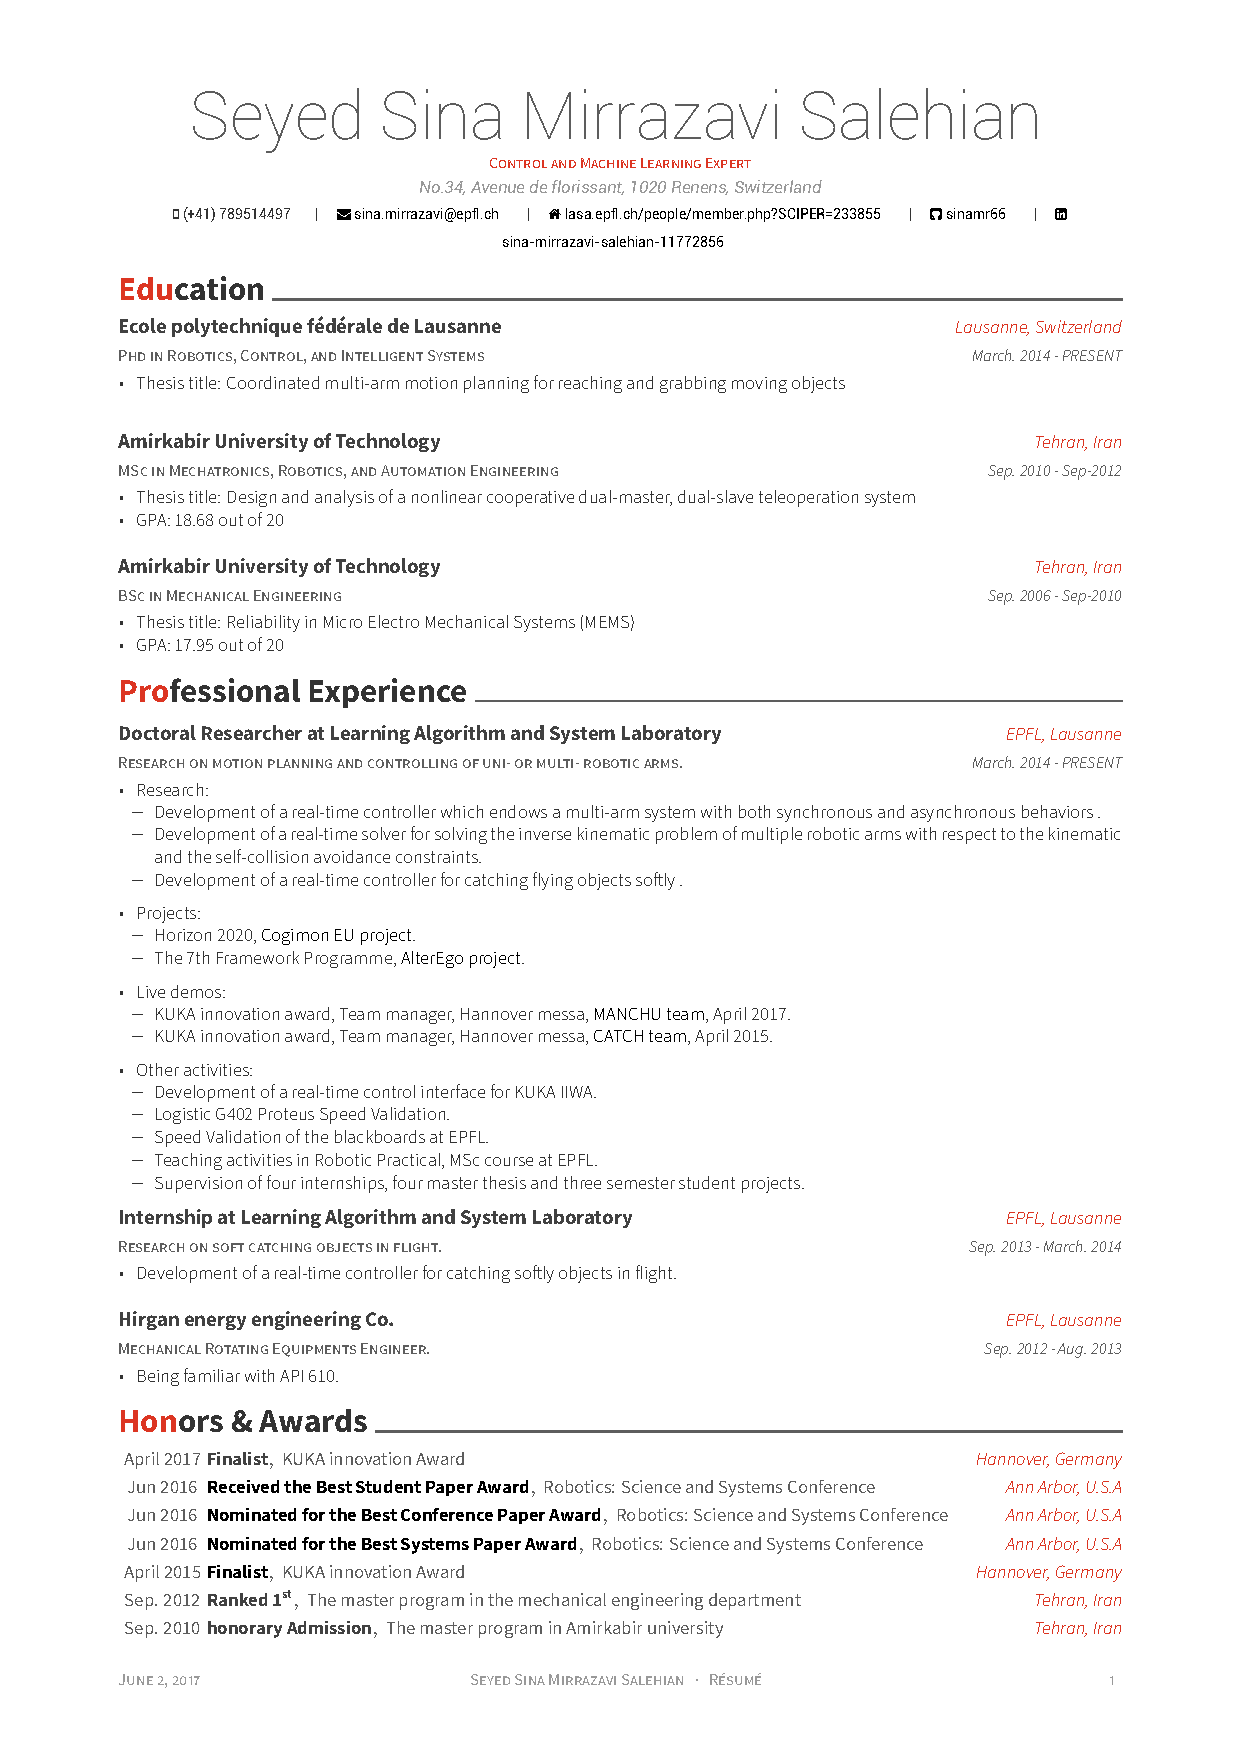
\includepdf[pages=-]{CV.pdf}
\fi

\end{document}